\documentclass[12pt]{amsart}
      % \newif\ifpreview
      % \previewfalse

% approx iid
\newcommand\simiid{\stackrel{\mathclap{\normalfont\mbox{\tiny{iid}}}}{\sim}}
\usepackage{natbib}
\usepackage{titlecaps}
\Addlcwords{a about above after again against all am an and any are aren't as at be because been before being below between both but by can't cannot could couldn't did didn't do does doesn't doing don't down during each few for from further had hadn't has hasn't have haven't having he he'd he'll he's her here here's hers herself him himself his how how's i i'd i'll i'm i've if in into is isn't it it's its itself let's me more most mustn't my myself no nor not of off on once only or other ought our ours ourselves out over own same shan't she she'd she'll she's should shouldn't so some such than that that's the their theirs them themselves then there there's these they they'd they'll they're they've this those through to too under until up very was wasn't we we'd we'll we're we've were weren't what what's when when's where where's which while who who's whom why why's with won't would wouldn't you you'd you'll you're you've your yours yourself yourselves}

% Fonts
% at some point figure out bolding ...
\usepackage[default,osfigures,scale=0.95]{opensans}
%\usepackage[sfdefault,scaled=.85]{FiraSans}
\usepackage[T1]{fontenc}
\usepackage{textcomp}
\usepackage[varqu,varl]{zi4}% inconsolata typewriter
\usepackage{amsmath,amsthm}
\usepackage[cmintegrals]{newtxsf}
\usepackage[T1]{fontenc}
\usepackage{ae}

% easy commands for number propers
\newcommand{\first}{1$^{\text{st}}$}
\newcommand{\second}{2$^{\text{nd}}$}
\newcommand{\third}{3$^{\text{rd}}$}
\newcommand{\nth}[1]{${#1}^{\text{th}}$}

% Generate some fake text
\usepackage{blindtext}

% % add watermark
% \usepackage{draftwatermark}
% \SetWatermarkText{Submission Copy}
% \SetWatermarkScale{.5}
% \SetWatermarkColor[gray]{0.9}

% layout control
\usepackage{geometry}
\geometry{verbose,tmargin=1in,bmargin=1.25in,lmargin=1in,rmargin=1in}
\usepackage{parallel}
\usepackage{parcolumns}
\usepackage{fancyhdr}
\usepackage[export]{adjustbox}
\usepackage{etoolbox}

% math typesetting
\usepackage{array}
\usepackage{amsmath}
\usepackage{amssymb}
\usepackage{amsthm}
\usepackage{amsfonts}
\usepackage{relsize}
\usepackage{mathtools}
\usepackage{bm}
%\usepackage[%decimalsymbol=.,digitsep=fullstop]{siunitx}

% restricts float objects to be inserted before end of section
% creates float barriers
\usepackage[section]{placeins}

% tables
\usepackage{tabularx}
\usepackage{booktabs}
\usepackage{multicol}
\usepackage{multirow}
\usepackage{longtable}

% to adapt caption style
\usepackage[font={small},labelfont=bf]{caption}

% footnotes at bottom
%\usepackage[bottom]{footmisc}

% to change enumeration symbols begin{enumerate}[(a)]
\usepackage{enumerate}
\usepackage{paralist}

% to colorize links in document. See color specification below
\usepackage[pdftex,hyperref,x11names]{xcolor}

% for multiple references and insertion of the word "figure" or "table"
% \usepackage{cleveref}

% load the hyper-references package and set document info
\usepackage[pdftex]{hyperref}

% graphics stuff
\usepackage{subfigure}
\usepackage{graphicx}
\usepackage[space]{grffile} % allows us to specify directories that have spaces
\usepackage{placeins} % prevents floats from moving past a \FloatBarrier
\usepackage{tikz}

% sideway figures
\usepackage{rotating}
\usepackage{lscape}

%\usepackage[figuresright]{rotating}
% \newenvironment{amssidewaysfigure}  {\begin{sidewaysfigure}\vspace*{.8\textwidth}\begin{minipage}{\textheight}\centering}
%   {\end{minipage}\end{sidewaysfigure}}

% Spacing
\usepackage[doublespacing]{setspace}

% outside code
\usepackage{listings}
\usepackage{enumitem}

% define clickable links and their colors
\hypersetup{%
	unicode=false,          % non-Latin characters in Acrobat's bookmarks
	pdftoolbar=true,        % show Acrobat's toolbar?
	pdfmenubar=true,        % show Acrobat's menu?
	pdffitwindow=false,     % window fit to page when opened
	pdfstartview={FitH},    % fits the width of the page to the window
	pdfnewwindow=true,%
	%pagebackref=false,%
	pdfauthor={Shahryar Minhas, et alia.},%
	pdftitle={Taking Dyads Seriously},%
	colorlinks,%
	citecolor=black,%
	filecolor=black,%
	linkcolor=black,%
	urlcolor=RoyalBlue4
}

% -------------------- title -------------------- %

\title{Taking Dyads Seriously}
\vspace{\baselineskip}

% \author[Minhas]{Shahryar Minhas}
% \address{Shahryar Minhas: Department of Political Science}
% \curraddr{Michigan State University}
% \email[Corresponding author]{minhassh@msu.edu}

% \author[Dorff]{Cassy L. Dorff}
% \address{Cassy L. Dorff}
% \curraddr{Department of Political Science, University of New Mexico}
% \email{cdorff@unm.edu}

% \author[Foster]{Margaret Foster}
% \address{Margaret Foster}
% \curraddr{Department of Political Science, Duke University}
% \email{margaret.foster@duke.edu}

% \author[Gallop]{Max Gallop}
% \address{Max Gallop}
% \curraddr{Department of Government and Public Policy, University of Strathclyde}
% \email{max.gallop@strath.ac.uk}

% \author[Liu]{Howard Liu}
% \address{Howard Liu}
% \curraddr{Department of Political Science, Duke University}
% \email{hao.liu@duke.edu}

% \author[Tellez]{Juan Tellez}
% \address{Juan Tellez}
% \curraddr{Department of Political Science, Duke University}
% \email{juan.tellez@duke.edu}

% \author[Ward]{Michael D. Ward}
% \address{Michael D. Ward}
% \curraddr{Department of Political Science, Duke University}
% \email{michael.d.ward@duke.edu}

% \date{\today}

% \thanks{Shahryar Minhas and Michael D. Ward acknowledge support from National Science Foundation (NSF) Award 1259266. Peter Hoff, John Ahlquist, Robert Franzese, Arturas Rozenas, Betsy Sinclair, Jacob Montgomery and Benjamin Appel provided welcome and helpful comments. We also thank Douglas Gibler for kindly providing us with a copy of the data and programs he used in \citet{gibler:2017}. We benefited from presentations of this material at the 2017 Political Methodology Conference, and our home institutions.}

\setlength{\headheight}{15pt}
\setlength{\headsep}{20pt}
\pagestyle{fancyplain}
\fancyhf{}
\lhead{\fancyplain{}{}}
% \chead{\fancyplain{}{Taking Dyads Seriously}}
\chead{\fancyplain{}{}}
% \rhead{\fancyplain{}{\today}}
\rhead{\fancyplain{}{}}
\rfoot{\fancyplain{}{\thepage}}

% references to graphics
\makeatletter
% \def\input@path{{/Users/janus829/Dropbox/toDo_notes/nsfSumm/Graphics/}, {/Users/s7m/Dropbox/toDo_notes/nsfSumm/Graphics/}}
% \graphicspath{{/Users/janus829/Dropbox/toDo_notes/nsfSumm/Graphics/}, {/Users/s7m/Dropbox/toDo_notes/nsfSumm/Graphics/}}

% easy command for boldface math symbols
\newcommand{\mbs}[1]{\boldsymbol{#1}}

% command for R package font
\newcommand{\pkg}[1]{{\fontseries{b}\selectfont #1}}

% Add some colors
\definecolor{red1}{RGB}{253,219,199}
\definecolor{red2}{RGB}{244,165,130}
\definecolor{red3}{RGB}{178,24,43}

\definecolor{green1}{RGB}{229,245,224}
\definecolor{green2}{RGB}{161,217,155}
\definecolor{green3}{RGB}{49,163,84}

\definecolor{blue0}{RGB}{255,247,251}
\definecolor{blue1}{RGB}{222,235,247}
\definecolor{blue2}{RGB}{158,202,225}
\definecolor{blue3}{RGB}{49,130,189}
\definecolor{blue4}{RGB}{4,90,141}

\definecolor{purple1}{RGB}{191,211,230}
\definecolor{purple2}{RGB}{140,150,198}
\definecolor{purple3}{RGB}{140,107,177}

\definecolor{brown1}{RGB}{246,232,195}
\definecolor{brown2}{RGB}{223,194,125}
\definecolor{brown3}{RGB}{191,129,45}

% square bracket matrices
\let\bbordermatrix\bordermatrix
\patchcmd{\bbordermatrix}{8.75}{4.75}{}{}
\patchcmd{\bbordermatrix}{\left(}{\left[}{}{}
\patchcmd{\bbordermatrix}{\right)}{\right]}{}{}


\begin{document}
% \ifpreview {
%    \definecolor{personal}{rgb}{1.0, 1.0, 0.0}
%    \pagecolor{personal}
%    }
% \fi


\small{\singlespacing{
\begin{abstract}
International relations scholarship concerns dyads, yet standard modeling approaches fail to adequately capture the data generating process behind dyadic events and processes. As a result, they suffer from biased coefficients and poorly calibrated standard errors. We introduce a regression-based approach, the Additive and Multiplicative Effects (AME) model, that better accounts for the inherent dependencies in dyadic data. First, we conduct a simulation to highlight how the model captures dependencies and show that accounting for these processes improves our ability to conduct inference on dyadic data. Second, we compare the AME model to approaches used in three prominent studies from recent international relations scholarship. For each study, we find that compared to AME, the modeling approach used performs notably worse at capturing the data generating process. Further, conventional methods misstate the effect of key variables and the uncertainty in these effects. Finally, AME outperforms standard approaches in terms of out-of-sample fit. In sum, our work shows the consequences of failing to take the dependencies inherent to dyadic data seriously. Most importantly, by better modeling the data generating process underlying political phenomena, the AME framework improves scholars' ability to conduct inferential analyses on dyadic data.
\end{abstract}
}}


\maketitle

\begin{center}
	\textbf{Word count}: 9,177
\end{center}

\thispagestyle{empty}
\newpage\setcounter{page}{1}

\section{\textbf{Introduction}}

\citet{aronow:etal:2015} estimate that during the period 2010 to 2015, over sixty articles were published in the \textit{American Political Science Review}, \textit{American Journal of Political Science}, and \textit{International Organization} using dyadic data.\footnote{In 2017, \textit{International Studies Quarterly} published a special issue on Dyadic Research Designs along with an online symposium to discuss the papers.} Most of these studies use a generalized linear model (GLM).  However, this approach to studying dyadic data increases the chance of faulty inferences by assuming data are conditionally independent and identically distributed (iid). Most standard approaches assume that the problems raised by non-iid relational data can be addressed by recalculating the standard errors of estimated parameters to reflect the potential clustering of cases. In practice, such strategies rarely work because they do not directly address the fundamental data generating process. This is important to consider since the inferential problems caused by non-iid  observations affect more than just diagonals of the variance co-variance matrix \citep{beck:2012,franzese:hays:2007,king:roberts:2014}.

In this article, we discuss how the Additive and Multiplicative Effects (AME) model can be used to model the interdependencies underlying the data generating process of dyadic structures \citep{hoff:2008,minhas:etal:2018}. We focus on three types of interdependencies that can complicate dyadic analyses. First, dependencies may arise within a set of dyads if a particular actor is more likely to send or receive actions such as conflict.\footnote{In the case of undirected data where there is no clear sender or receiver, it is still essential to take into account the variance in how active actors are in the system.} Additionally, if the event of interest has a clear sender and receiver, we are likely to observe dependencies within a dyad; for example, if a rebel group initiates a conflict against a government, the government will likely reciprocate that behavior. We capture these effects, often referred to as first- and second-order dependencies, respectively, within the additive effects portion of the model. Third-order dependencies capture relationships of transitivity, balance, and clusterability between different dyads. For example, we can only understand why Poland was involved in a dyadic conflict with Iraq in 2003 if we understand that the United States invaded Iraq in 2003 and that Poland often participates in US-led coalitions. The multiplicative effects capture these sorts of dependencies, especially those that result because the specified model has not accounted for a latent set of shared attributes that affect actors' probability of interacting with one another.

We begin with a discussion of these dependencies and an introduction to the AME model. Next, we conduct a simulation study to show how the AME approach can recover unbiased and well-calibrated regression coefficients in the context of dyadic data. Last, to highlight the utility of this approach, we apply the AME model to three recent studies in the international relations (IR) literature. Our comparison reveals that by accounting for observational dependence, AME produces more precise estimates and better-calibrated confidence intervals for key variables. Consequently, AME generates results that, at times, differ from those found in the original study as well as from the broader literature. Moreover, we demonstrate that the AME latent factor approach offers substantive insights that are often occluded by ignoring the interdependencies found in the relational data widely employed in IR. Finally, we show that for each replication our network-based approach provides substantially more accurate out-of-sample predictions than the models used in the original studies.

The AME approach advances statistical analysis of dyadic data by accounting for observational dependence while allowing scholars to test the substantive effect of variables of interest. Thus, the AME allows scholars to achieve a two-fold goal: to continue to generate meaningful, substantive insights about political phenomena without abandoning a regression based approach, while at the same time accounting for the data generating processes behind such events of interest. Most importantly, the AME approach concentrates on the relational aspect of the field of international relations through a statistical framework that is familiar to most scholars.

\section{\textbf{Dependencies in Dyadic Data}}

In thinking about dyadic data, scholars in the field begin by structuring it as a set of dyadic observations stacked on top of one another. Each observation is assumed to be independent of the others. Thus, for example, a conflict sent from actor the United States to Japan, is assumed to be independent of any action that Japan may send to the United States. Additionally, every action sent by Japan to others in the system is considered independent even though each of those interactions involves a common sender, i.e, Japan. As a result, the assumption that most begin with is that each dyadic interaction is taking place in isolation of the others. 

\begin{table}[ht]
	\captionsetup{justification=raggedright }
	\centering
	\begin{minipage}{.45\textwidth}
		\centering
		\begingroup
		\setlength{\tabcolsep}{10pt}
		\begin{tabular}{ccc}
			Sender & Receiver & Event \\
			\hline\hline
			$i$ & $j$ & $y_{ij}$ \\
			\multirow{2}{*}{\vdots} & $k$ & $y_{ik}$ \\
			~ & $l$ & $y_{il}$ \\
			$j$ & $i$ & $y_{ji}$ \\
			\multirow{2}{*}{\vdots} & $k$ & $y_{jk}$ \\
			~ & $l$ & $y_{jl}$ \\
			$k$ & $i$ & $y_{ki}$ \\
			\multirow{2}{*}{\vdots} & $j$ & $y_{kj}$ \\
			~ & $l$ & $y_{kl}$ \\
			$l$ & $i$ & $y_{li}$ \\
			\multirow{2}{*}{\vdots} & $j$ & $y_{lj}$ \\
			~ & $k$ & $y_{lk}$ \\
			\hline\hline
		\end{tabular}
		\endgroup
		\caption{Structure of datasets used in canonical design.} 
		\label{tab:canDesign}
	\end{minipage}
	$\mathbf{\longrightarrow}$
	\begin{minipage}{.45\textwidth}
		\centering
		\begingroup
		\setlength{\tabcolsep}{10pt}
		\renewcommand{\arraystretch}{1.5}
		\begin{tabular}{c||cccc}
		~ & $i$ & $j$ & $k$ & $l$ \\ \hline\hline
		$i$ & \footnotesize{NA} & $y_{ij}$ & $y_{ik}$ & $y_{il}$ \\
		$j$ & $y_{ji}$ & \footnotesize{NA}  & $y_{jk}$ & $y_{jl}$ \\
		$k$ & $y_{ki}$ & $y_{kj}$ & \footnotesize{NA}  & $y_{kl}$ \\
		$l$ & $y_{li}$ & $y_{lj}$ & $y_{lk}$ & \footnotesize{NA}  \\
		\end{tabular}
		\endgroup
		\caption{Adjacency matrix representation of data in Table~\ref{tab:canDesign}. Senders are represented by the rows and receivers by the columns. }
		\label{tab:netDesign}
	\end{minipage}
\end{table}

\FloatBarrier

To start to move away from this assumption and better understand the dependencies that emerge in relational data it is helpful to shift towards structuring dyadic data in the form of an adjacency matrix as shown in the top right of Table~\ref{tab:netDesign}. Here rows designate the senders of an event and columns the receivers. The cross-sections in this matrix represent the action that was sent by an actor on the row to one designated in the column. Thus $y_{ij}$ designates an action, such as a conflictual event or trade flows, that is sent from actor $i$ to actor $j$. 

Using the structure of an adjacency matrix we can visualize the types of first and second order dependencies that complicate the analysis of relational data in traditional GLMs. Figure~\ref{fig:adjMatDeps} clarifies the types of dependencies that can manifest in these types of data structures. The adjacency matrix on the top left highlights a particular row of an adjacency matrix, to illustrate that values across a particular row of an adjacency matrix may be more similar to each other than other values in the adjacency matrix because each of these values has a common sender. Homogeneity in interactions involving a common sender also manifest heterogeneity in how active actors are across the network when compared to each other. Thus in most relational datasets (e.g., trade flows, conflict, participation in international organizations, even networks derived from Twitter or Facebook) we often find that there are some actors who are much more active than others \citep{barabasi:reka:1999}. Unless one is able to develop a model that can account for the variety of explanations that may play a role in determining why a particular actor may be more active than others, parameter estimates from standard statistical models will be biased.

\begin{figure}
	\begin{tabular}{cc}
		\texttt{Sender heterogeneity} & \texttt{Receiver Heterogeneity} \\
		\includegraphics[width=.45\textwidth]{adjRowDep.png} & \includegraphics[width=.45\textwidth]{adjColDep.png} \\
		\texttt{Sender-Receiver Covariance} & \texttt{Reciprocity} \\
		\includegraphics[width=.45\textwidth]{adjRowColCovar.png} & \includegraphics[width=.45\textwidth]{adjRecip.png} \\
	\end{tabular}
	\caption{Nodal and dyadic dependencies in relational data.}
	\label{fig:adjMatDeps}
\end{figure}

For similar reasons one also needs to take into account that there is a shared dependence between dyadic observations that share a common receiver. The bottom-left panel, illustrates that sender and receiver type dependencies can also blend together. Specifically, as actors who are more likely to send ties in a network tend to also be more likely to receive them. As a result, the rows and columns in an adjacency matrix are often correlated. For example, consider that trade flows both from and to many wealthy, developed countries. The bottom-right panel, highlights a second order dependence, specifically, reciprocity. This is a dependency occurring within dyads involving the same actors whereby values of $y_{ij}$ and $y_{ji}$ are correlated. The concept of reciprocity has deep roots in the study of relations between states \citep{richardson:1960,keohane:1989}. The purpose of highlighting each of these dependencies through the set of panels in Figure~\ref{fig:adjMatDeps} is to more easily visualize how each of these dependencies manifest in relational data. Alternatively, when we simply simply stack dyads in some arbitrary order, these dependencies are easy to ignore.

The dependencies discussed so far involve at most dependence between two actors. For most relational data, however, dependencies do not simply manifest at this level. More often we find significant evidence of higher order structures that result from dependencies between multiple groups of actors. These dependencies arise because there may be a or some set of latent attributes between actors that affects their probability of interacting with one another \citep{wasserman:faust:1994,zinnes:1967}. In Figure~\ref{fig:thirdDeps} we provide a visualization of a hypothetical relational dataset. Here the nodes designate actors and edges between the nodes indicate that an interaction between the two took place. Each node is colored by the latent group to which they belong. 

\begin{figure}[ht]
	\includegraphics[width=.7\textwidth]{stochEquiv.pdf}
	\caption{Visualization of network with meso-scopic features.}
	\label{fig:thirdDeps}
\end{figure}

Clear from the visualization is that the actors belonging to the same group have a higher likelihood of having an interaction with each other than those from the other group. A prominent example of a network with this type of structure was found by \citet{adamic:glance:2005}, who visualized the ways in which right and left leaning political blogs linked to one another in the 2004 United States Election \citep{adamic:glance:2005}. They found that the degree of interaction between right and left leaning blogs was minimal, and that most of these blogs simply linked to those of their own ilk. This showcases the types of higher order dependencies that can emerge in relational data. First, the fact that interactions was determined by a shared attribute, in this case political ideology, is an example of homophily. Homophily can be used to explain the emergence of patterns such as transitivity (``a friend of a friend is a friend'') and balance (``an enemy of a friend is an enemy''), which also have a long history in international relations. The other major type of meso-scopic feature that emerges in relational data is community structure, which is often formalized through the concept of stochastic equivalence \citep{anderson:etal:1992}. This concept simply refers to the idea that groups of nodes that act similarly in the network are stochastically equivalent. In the example we have laid out above each of the left leaning blogs would be considered stochastically equivalent to one another. 

The major implication of the presence of homophily, stochastic equivalence, and the other dependencies we discussed above are that they complicate the practical assumption of observational independence. Inferences drawn from models that ignore potential interdependencies between dyadic observations face a number of well-known challenges: a) biased estimates of the effect of independent variables, b) uncalibrated confidence intervals, and c) poor predictive performance. By ignoring these potential interdependencies, we often ignore important features of the problem under study. The study of international relations is founded on the relations among actors. Why ignore the interdependencies that led to the study of IR in the first place?

% Thus, unless we specify a list of exogenous variables that determine this prevalence of triads, the probability of $j$ and $k$ forming a tie is not independent of the ties that already exist between those actors and others.

\section{\textbf{Additive and Multiplicative Effect Models for Networks}}

The AME approach can be used to conduct inference on cross-sectional and longitudinal networks with binary, ordinal, or continuous linkages. It is flexible and easy to use for analyzing the kind of relational data often found in social science. It accounts for nodal and dyadic dependence patterns, as well as higher-order dependencies such as homophily and stochastic equivalence.  We do not know whether interdependence dominates international relations, but as noted by Thoreau in reference to rumors that dairymen on strike were watering down milk: ``\ldots some circumstantial evidence is very strong, as when you find a trout in the milk.'' At a very minimum, it is necessary to examine whether there is interdependence since it challenges substantive arguments as well as statistical modeling \citep{snijders:2011}. 

Further parameter interpretation in the AME framework is straightforward because it has a simple regression basis as shown in Equation~\ref{eqn:ame} which portrays directed matrix \:

\begin{align}
\begin{aligned}
	y_{ij} &= g(\theta_{ij}) \\
	&\theta_{ij} = \bm\beta^{\top} \mathbf{X}_{ij} + e_{ij} \\
	&e_{ij} = a_{i} + b_{j}  + \epsilon_{ij} + \alpha(\textbf{u}_{i}, \textbf{v}_{j}) \text{  , where } \\
	&\qquad \alpha(\textbf{u}_{i}, \textbf{v}_{j}) = \textbf{u}_{i}^{\top} \textbf{D} \textbf{v}_{j} = \sum_{k \in K} d_{k} u_{ik} v_{jk}. \\
\label{eqn:ame}
\end{aligned}
\end{align}

With this framework, it is straightforward to model dyadic observations as conditionally independent given $\bm\theta$, where $\bm\theta$ depends on the the unobserved random effects modeled to account for the potential \first, \second, and \third-order dependencies. In Equation~\ref{eqn:srmCov}, $a_{i} + b_{j}  + \epsilon_{ij}$ represent the additive random effects in this framework and account for sender, receiver, and within-dyad dependence. The multiplicative effects, $\textbf{u}_{i}^{\top} \textbf{D} \textbf{v}_{j}$, capture higher-order dependence patterns in $\bm\theta$ after accounting for any known covariate information.\footnote{This procedure is described in detail in \citet{hoff:2008} and \citet{minhas:etal:2016:arxiv}. A Bayesian procedure in which parameters are iteratively updated using a Gibbs sampler is described in the appendix.}

\section{\textbf{Simulation study}}

We utilize a simulation study to highlight the utility of AME as an inferential tool for dyadic analysis.\footnote{Alternative network based approaches for dyadic data are exponential random graph models (ERGMs) and the related stochastic actor oriented model (SAOM). While both these models have led to numerous contributions to a variety of literatures, the applicability of these approaches may be limited to certain types of networks and individual level characteristics. Specifically, \citet{block:etal:2017} note that these types of  models may not be appropriate in situations where network and behavioral data depend on unobserved latent variables, which is explicitly the focus of our analysis here.} Most scholars working with dyadic data are primarily concerned with understanding the effect of a particular independent variable on a dyadic dependent variable. The goal of the simulation is to assess how well AME can provide unbiased and well-calibrated estimates of coefficient parameters in the presence of unobserved dependencies. Specifically, we are concerned with conducting inference on regression parameters of a linear model for a network in the case where there is an unaccounted for higher order dependence pattern. For instance, assume that the true data-generating process for a particular $Y$ is given by:

\begin{align}
	y_{i,j} \sim  \mu + \beta x_{i,j} + \gamma w_{i,j} + \epsilon_{i,j}
	\label{eqn:sim}
\end{align}

where $Y= \{y_{i,j}\}\in \mathbb R^{n\times n}$ is an observed sociomatrix, $X = \{x_{i,j} \} \in \mathbb R^{n \times n}$ is a matrix of observed dyad-specific characteristics, and $W = \{ w_{i,j}\} \in \mathbb R^{n \times n}$ is a matrix of unobserved dyad-specific characteristics. $Y$ can be thought of as a dyadic dependent variable, $X$ and $W$ are both dyadic covariates that are a part of the data-generating process for $Y$, but $W$ is not observed. We compare inference for $\mu$ and $\beta$---the latter parameter would be of primarily theoretical concern for applied scholars---using three models:

\begin{itemize}
	\item the ``standard'' international relations approach estimated through a typical generalized linear model; 
	\item the AME approach outlined in the previous section with a unidimensional latent factor space ($K=1$);\footnote{Results with higher values of $K$ are similar.}
	\item and an ``oracle'' regression model that assumes we have measured all sources of dependencies and thus includes both $x_{i,j}$ and $w_{i,j}$. 
\end{itemize}

The first model corresponds to the ``standard'' approach in which little is explicitly done to account for dependencies in dyadic data. In the second model, we use the AME framework described in the previous section. For both the first and second models, we are simply estimating a linear model of $X$ on $Y$, and assessing the extent to which inference on the regression parameters are complicated in the presence of unobserved dependencies, $W$. In the last model, we provide an illustration of the ideal case in which we have observed and measured $W$ and include it in our specification for $Y$. The oracle case provides an important benchmark for the standard and AME approaches.

For the simulation we set the true value of $\mu$ (the intercept term) to -2 and $\beta$ (the effect of $X$ on $Y$) to 1.\footnote{The value of $\gamma$ is also set to 1, which corresponds to an example where the $W$ character is associated with homophily.} We conduct two sets of simulations, one in which the number of actors in the network is set to 50 and the other at 100. In total, we ran 1,000 simulations where we begin by simulating $Y$ from the specification given in Equation~\ref{eqn:sim} and then for each simulated $Y$ we estimated a standard, AME, and oracle model. 

We compare the performance of the models first in terms of how well they estimate the true values of $\mu$ and $\beta$ in Figure~\ref{fig:ameBias} by depicting the average $\mu$ and $\beta$ estimates from the simulations for the three models. The panels in the left show the results for when the number of actors is set to 50 and those on the right for 100; and the top pair of panels represents the estimates for $\mu$ while the bottom pair do the same for $\beta$. In each case, we find that the estimates for $\mu$ and $\beta$ produced by the standard approach are notably off from their true values. On the other hand, the AME model performs just as well as the oracle case in estimating the true parameter values. 

\begin{figure}
	\centering
	\caption{Regression parameter estimates for the standard, AME, and oracle models from 1,000 simulations. Summary statistics are presented through a traditional box plot, and the estimates from each simulation are visualized as well as points.}
	\label{fig:ameBias}
	\includegraphics[width=1\textwidth]{graphics/ameSimBias_all.pdf} \\
\end{figure}

Next, we estimate the 95\% confidence interval for the three models in each of the simulations and estimate the proportion of times that the true value fell within those intervals. The results are summarized in Figure~\ref{fig:ameCalib}, and again we see that the AME approach performs as well as the oracle, while the standard approach performs poorly by comparison. The implication of the results presented in Figures~\ref{fig:ameBias} and ~\ref{fig:ameCalib} is that standard approaches can often fail at estimating parameter values and conducting inferential tasks in the presence of unobserved dependencies. The AME approach by comparison can be used as a tool for scholars working with dyadic data to still estimate the true effects of their main variables of interest, while accounting for dependencies that do often emerge in dyadic data. 

\begin{figure}
	\centering
	\caption{Proportion of times the true value fell within the estimated 95\% confidence interval for the standard, AME, and oracle models from 1,000 simulations.}
	\label{fig:ameCalib}
	\includegraphics[width=1\textwidth]{graphics/ameSimCover_all.pdf} \\
\end{figure}

Moreover, the AME approach allows scholars to better understand what parameters their model may be missing. In the case of the simulation here, $W$ is set as an unobserved dyadic covariate that had a homophilous effect on $Y$. Homophilous because $W$ within this framework is simply an example of a dyadic attribute involving $i$ and $j$ that positively affects the degree to which they will interact with one another, i.e., $y_{ij}$. This type of unobserved dependency will be captured through the multiplicative effects portion of the model, $\mathbf{U}^{\top} \mathbf{D} \mathbf{V}$. To estimate how well the model performs, we recover the multiplicative effects term for each simulation and calculate the correlation between it and the unobserved dependency, $W$.\footnote{Specifically, since both the multiplicative effects term and $W$ are continuous dyadic variables, we calculate the Pearson correlation coefficient.} We visualize the distribution of the correlations from each of the 1,000 simulations in Figure~\ref{fig:ameCorr} for the case where the number of actors is set to 100 (top pair of panels) and 50. Additionally, we calculate the median across the correlations and display the result using a vertical line. For both $n=50$ and $n=100$, we find that the multiplicative effects perform very well in capturing the unobserved dependency, which indicates that this framework is not simply capturing noise but can be used as a tool to estimate unobserved structure. 

\begin{figure}
	\centering
	\caption{Distribution of correlation between missing variable and multiplicative random effect in AME across the 1,000 simulations. Vertical line through the distribution represents the median value across the simulations.}
	\label{fig:ameCorr}
	\includegraphics[width=1\textwidth]{graphics/ameSimCorr.pdf} \\
\end{figure}

What this simulation has shown is that beyond obtaining less biased and better-calibrated parameter estimates, a key benefit of the AME framework is to directly estimate unobserved dependencies through the random effects structure of the model. Scholars can use this framework in an iterative fashion: beginning with an estimated a model, they can then empirically study the structure of the random effects to assess whether there are unobserved covariates that they want to include in their models. At the very least, what this simulation section shows is that the AME model can help in estimating the true effect and conducting inference on the independent variables that scholars have operationalized to test their theoretical propositions.

\section{Re-estimation with AME}
 
\subsection{Design}

We choose five prominent studies from the broad field of international relations and international political economy that utilize relational data \citep{reiter:stam:2003, mcdonald:2004,  rose:2004, weeks:2012, gibler:2017}. These studies are recent and have been cited over 100 times. Each of these pieces was published in a prominent journal and is well-known in the literature. Each used the standard approach in political science, which is to employ some form of a general linearized regression that ignores dyadic interdependencies, except as they may reveal themselves in included variables. Also part of the gold standard is a post estimation cleanup thought to be a palliative, and each of these studies adjust the posterior standard errors in an attempt to account for the clustering of observations.

\begin{table}
\caption{Features of the Studies Re-estimated. }
	\begin{tabular}{lcccccc}
		& Model &  Date Range & N. Actors  & N. Dyads & Dyads Type & Clustering $\sigma_{\hat{\beta}}$ \\ \toprule
		Reiter \& Stam (2003) &Logit &1945--1995 &  193 & $753,456$ & Directed & Robust \\	
		McDonald (2004) & Logit &1959--2002 & 198 & $92,354$ & Undirected & Robust\\
		Rose (2004) & OLS & 1948--1999 & 177 & $234,597$ & Directed & Robust \\	 
		Weeks (2012) & Logit & 1946--1999 &197 &  $901,540$ & Directed & Robust \\
		Gibler (2017) & Logit & 1816--2008 &193 &   $650,557$ & UnDirected & none \\ \bottomrule
	\end{tabular}
\end{table}

We obtained the data for each of these studies from their replication archives and replicated the main results of each of the articles.\footnote{Without exception this was straightforward to accomplish, thanks to an increasing norm in the social sciences of open data sharing.} We also examine each of the models using the AME framework described above.  Our goal is to ascertain whether the ignored interdependencies -- the non-iid structure of the relational data -- would result in different model estimates when they were addressed in an AME framework, and more importantly to see if there were substantive opportunities that were presented with the dynamic factor approach.  
Finally, in each study we assess whether there is any new substantive finding that emerges or indeed if any disappear once the interdependencies in the data are modeled.

The broader goal, beyond introducing the use of the AME framework in an applied setting, is to examine the extent to which interdependencies within typical dyadic data make much difference in what we have learned about international relations from recent empirical studies that use a framework that ignores dependencies.  Based in part our our results as well as the statistical and mathematical characteristics of the AME framework, we believe that it does. The dynamic latent factor model provides a step forward in the modeling of international relations.

Given current practices, most scholars have a single variable in a complicated empirical model that they look at for evaluating the validity of their empirically estimated models.  Whether putative control variables, for example, are precisely estimated is less important. Generally, interpretations focus on a small set of independent variables.  In the study by Reiter and Stam (2003) the main question is to determine in mixed dyads -- consisting of a democratic country and country ruled by a personalist dictatorship -- whether it is the democratic country or the personalist country that is associated with a greater likelihood that the dyad is in a dispute.  In a regression including fourteen coefficients, they focus on whether the variables that capture whether the initiator is a democratic country are statistically significant.\footnote{In particular, the variables \texttt{Pers/Democ} and \texttt{Democ/Pers} in Model 3, in Table 1, page 335.} In our evaluation we focus on the same question in the re-examination of the Reiter and Stam study to determine whether the model replicates when re-estimated within the AME framework. Each of the other four studies also has a crucial finding that we hone in on to further draw into focus the potential differences brought about by utilizing an AME estimation procedure.  In Table~\ref{tab:modelFindingSumm}, we present the overall results; the term \textit{does not replicate} indicates only that the sign and/or significance of the putatively crucial finding in the original study is not also found in the AME estimation.

\begin{table}[ht]
\centering
\caption{Here we provide a brief summary of the key variable in each of the five replications and a note about whether or not the finding is replicated when using our network based approach. Cases in which the substantive finding is not replicated are highlighted in bold.}
	\begin{tabular}{l p{7cm} l} \toprule
		\multirow{2}{*}{Study} & \multirow{2}{*}{Central Finding} &  Replicates \\ 
			& &  in a Network Model? \\ \toprule
		Reiter \& Stam (2003) & Personalist Regimes Attack Democracies, Not Vice Versa & {Replicates} \\ \midrule
		McDonald (2004) & Lower Trade Barriers and Higher Trade Lead to Peace & {Does Not Replicate}\\ \midrule
		Rose (2004) & WTO Membership Does not Effect Trade & {Replicates}\\ \midrule
		Weeks (2012) & Bosses, Juntas and Strongmen are more Aggressive, Machines are Not & {Does Not Replicate} \\\midrule
		Gibler (2017) & Power Parity at Time of Entry to International System Inceases Conflict & {Does Not Replicate} \\ \bottomrule
	\end{tabular}
	\label{tab:modelFindingSumm}
\end{table}

In addition, we also examine the predictions made with each approach using an out-of-sample cross validation strategy. By accounting for exogenous and network dependent patterns that give rise to conflict systems we are able to better account for the data generating process underlying relational data structures. To show that this is the case, we examine whether our approach achieves better predictive performance in an out-of-sample context than traditional dyadic models. To evaluate our model, we randomly divide the $\binom n 2 \times T$ data values into $k=30$ sets, letting $s_{ij,t}$ be the set to which pair $ij,t$ is assigned. Then for each $s \in \{1,\ldots,k\}$, we:

\begin{enumerate}
	\item estimate model parameters with $\{y_{ij,t}: s_{ij,t} \neq s\}$, the data not in set $s$,
	\item and predict $\{\hat{y}_{ij,t}: s_{ij,t} = s\}$ from these estimated parameters. 
\end{enumerate}

\noindent The result of this procedure is a set of sociomatrices $\bm \hat Y$, in which each entry $\hat y_{ij,t}$ is a predicted value obtained from using a subset of the data that does not include $y_{ij,t}$. 

We set a number of benchmarks for comparison. First, we compare the AME model to a GLM model (that used in the original study) using the same covariates to show the effect of accounting for network dependencies on predicting conflict. We supplement this with an alternative GLM that includes not just these covariates, but also a lagged dependent variable and a lagged reciprocity term. The lagged dependent variable is the equivalent of saying that conflict and peace are relatively likely to persist between dyads, while the inclusion of a lagged reciprocity term in a GLM framework is a simple way to account for retaliatory strikes.

We utilize three performance criteria to compare the models: Receiver Operator Characteristic (ROC) curves, Precision Recall (PR) curves, and separation plots. ROC curves look at the trade-off between true positive rates and false positive rates at different thresholds of classification. An issue with an ROC Curve when looking at conflict, is that it is relatively rare at the dyadic level: in most years only 3\% of possible dyads are in conflict with one another. If peace is common, even a poor model will have a very low False Positive Rate. The ROC curves are best for balanced samples with as many events as non-events. To better assess which models predict the presence of conflict, not just its absence, we look at PR Curves. These examine the trade-offs between the percentage of conflicts a model predicts, and the percentage of predicted conflicts which occur. Lastly, we examine separation plots \citep{greenhill:etal:2011}. These provide an intuitive visualization of the accuracy of our predictions by juxtaposing a line showing the predicted probability of conflict with whether conflict actually occurs for all cases (where the cases are sorted by the predicted probability and then colored to indicate the outcome). Here a perfect model would have all cases where conflict actually exists on the right with a predicted probability of $1$, and would predict $0$ in all other cases. All of the models' performance out of sample by these metrics are displayed in figure \ref{fig:roc_ame}. The AME model with covariates is the best performing model out of sample in all cases. This model outperforms each of the GLM variants by a notable margin.

\begin{table}[ht]
\centering
	\begin{tabular}{l|l cc}
	~ & ~ & GLM & AME \\
	\toprule
\multirow{2}{*}{Reiter \& Stam (2003)} & Area Under ROC Curve, AUC-ROC & 0.92 & {0.96} \\
		~ & Area Under PR Curve, AUC-PR & 0.08 &  {0.15} \\		\midrule
\multirow{2}{*}{McDonald (2004)} & AUC-ROC & 0.92 &  {0.99} \\
		~ & AUC-PR & 0.13 &  {0.28} \\		\midrule
\multirow{2}{*}{Rose (2004)} & Root Mean Squared Error RMSE & 3.23 &  {1.99} \\
		~ & Root Median Squared Error RMDSE & 2.01 &  {1.06} \\	\midrule
\multirow{2}{*}{Weeks (2012)} & AUC-ROC & 0.64 &  {0.97} \\
		~ & AUC-PR & 0.00 &  {0.15} \\		\midrule
\multirow{2}{*}{Gibler (2017)} & AUC-ROC & 0.52 &  {0.91} \\
		~ & AUC-PR & 0.00 &  {0.08} \\			\bottomrule
	\end{tabular}
	\caption{Here we provide a summary of the out-of-sample performance based on our cross-validation strategy for each of the five replications when using the standard dyadic approach and our network based approach. Four of the five studies involved a binary dependent variable, so for those measures we provide area under the curve (AUC) statistics. The Rose study involved a Gaussian dependent variable and for that we use the root mean squared error (RMSE) and root median squared error (RMDSE). Cases in which our network based approach outperformed the standard approach are highlighted in bold.}
	\label{tab:modelPerfSumm}
\end{table}
\FloatBarrier

\subsection{Replication of Reiter \& Stam (2003)}

\citet{reiter:stam:2003} examine the relationship between democracy, dictatorship and the initiation of militarized disputes.  They use directed dyads and find that dyads involving a democratic leader on the one hand and a personalist dictator on the other tend to be violent. They also discover that dictators are likely to challenge democracies, but that this is not reciprocal.  In addition, military regimes and single-party regimes are more prone to initiate disputes with democracies, than the other way around.  They use the MID data, but note that ``We code a state as having initiated a dispute if it is on `side A' of a MID, the conventional approach to coding initiation. This means that the state was on the side that took the first action in the dispute, whether that action was the threat, display, or use of force. We code joiners as initiators or targets, though the results do not change if we do not code joiners as initiators or targets. \ldots Though coding initiation will always be difficult, the `side A' variable has been widely used in past conflict scholarship (page 334).'' Independent variables are largely taken from an earlier study and focus on various encodings of regime types, contiguity, alliance, and capability measures. As is prevalent in these kinds of studies, Reiter \& Stam employ a logistic regression that includes an indicator of the time since the last dispute as well as three cubic splines. The database for this study is constructed using EUGene \citep{bennett:stam:2000} and comprises approximately three-quarters of a million stacked dyads. Based on their statistical analysis, they conclude that institutional constraints affect the propensity of democratic and non-democratic leaders to engage in military conflict. 

In the original model, the variable ``Pers/Democ Directed Dyad" (which represents a Personalist $\rightarrow$ Democractic directed dyad) is clearly positive while the variable ``Democ/Personalist Directed Dyad'' is zero and the difference between the two coefficients is clearly distinct from zero. In our re-estimation using the AME framework, we also find that Pers-Democ directed dyad has a positive effect with zero excluded from the 95\% confidence interval while Democ-Pers directed dyad is indistinguishable from zero. Using this model, however, we can no longer conclusively say that the Pers/Democratic coefficient is larger than the Democ/Personalist one. Our re-estimation using the AME approach therefore cast some doubt on Reiter \& Stam's key claim that MIDs initiated by personalist dictatorships against democracies are more likely than MIDS initiated by democracies. Further, the effect of most of the covariates in the literature thought to predict interstate MIDs are much closer to zero when using the AME framework. Finally, our modeling approach outperforms the original model by better, and more accurately, predicting MIDs out-of-sample (Figure~\ref{fig:reitaucpr}).  

\begin{figure}
	\centering   
	\subfigure[AUC]{\label{fig:reitaucpr}\includegraphics[width=.45\textwidth]{reiter_stam_roc_outSample.pdf}}
	\subfigure[Precision and Recall]{\label{fig:reitpr}\includegraphics[width=.45\textwidth]{reiter_stam_pr_outSample.pdf}}
	\caption{Assessments of out-of-sample predictive performance for Reiter \& Stam (2003) using ROC curves and PR curves.}
\end{figure}
\FloatBarrier

\subsection{Replication of McDonald (2004)}

\citet{mcdonald:2004} studies whether trade promotes peace between nations. The link between conflict and trade is perplexing, with many persistent, yet competing explanations. \citet{mcdonald:2004} includes the argument that interdependence between states ``makes conflict less likely because of its efficiency over conquest in acquiring resources\ldots (547)''. Accordingly, his primary contribution is to provide evidence challenging the generalized linkage between peace and trade and to offer a new measurement of the key independent variable, trade. \citet{mcdonald:2004} refines the trade variable, arguing that \textit{free} trade, rather than trade alone, reduces the likelihood of conflict between states. His key hypothesis that greater levels of protection increase the probability of interstate conflict, an argument that builds on the work of classic liberalism and connects free trade to the power of domestic audiences. \citet{mcdonald:2004} measures free trade in two ways. The first captures the idea that larger protected sectors generate greater societal pressures resulting in pockets of support for war. This protection variable measures the proportion of customs revenue divided by total imports in the state that possesses the greater such ratio in each dyad. This measure captures the score of the state in the dyad that possesses higher barriers to trade (560). \citet{mcdonald:2004} also includes a measure of economic integration  calculated as ``the lower proportion of total dyadic trade (imports plus exports) divided by state $i$'s GDP or total dyadic trade divided by state $j$'s GDP'' (560). The binary, dependent variable is the onset of a new militarized interstate dispute within a given dyad. \citet{mcdonald:2004} employs logistic regression to examine the putative statistical significance of these variables. The models include splines to correct for temporal dependence, and robust standard errors clustered on each dyad.

% TO DO: include discussion and analysis of different K's in appendix (for M cD)

Our re-estimation with AME reveals that trade relations are highly interdependent and exhibit important patterns of transitivity.  Or, in other words, if countries $i$ and $j$ are highly dependent and countries $j$ and $k$ are also highly dependent, then we are likely to observe high dependency between countries $i$ and $k$. Our findings support those of Traag and Lupu (2013) which argue that indirect trade relations reduce the probability of conflict. This indicates that conflict is less likely between members of a trade community. Once we control for these dependencies, we can more clearly interpret the positive link between trade and conflict.  The most striking thing is that AME finds a positive conditional association between trade dependence and conflict ($\hat{\beta}= 18.4, \quad \sigma_{\hat{\beta}} = 28.6$), while the comparable numbers for the logistic regression found in the original articles are negative ($\hat{\beta}= -22.2, \quad \sigma_{\hat{\beta}} = 15.2$). At the same time, the AME has ROC and PR curves (shown in the Appendix) that dominate the results found in McDonald (2004).

\subsection{Replication of Rose (2004)}

In 2004, Andrew Rose published a study in the \textit{American Economic Review} \nocite{rose:2004} that proved to be quite controversial in terms of macroeconomic trade theory and in terms of trade policy in a variety of nations. It also provoked a number of responses in the international political economy literature \cite{tomz:etal:2007,ward:etal:2013}.  Rose's basic argument is that despite longstanding arguments made by trade theorists and the World Trade Organization that WTO membership fosters greater cooperation and thereby more trade among its members, the empirics do not bear out such claims. He uses a standard gravity model with dyadic data on bilateral merchandise trade (not services) for $175$ countries over a period of five decades. Estimating this model using OLS within many differing contexts, his conclusion was that: ``An extensive search reveals little evidence that countries joining or belonging to the GATT/WTO have different trade patters from outsiders \ldots (2004, page 98, abstract).''  The data for this study have been widely used in replications by many searching for the missing effects of the WTO -- as well as preferential trade agreements, bilateral investment theories, and other aspects of modern trade theory.  

When we compare the results of Rose's original OLS model to the AME model accounting for network dependencies, the results are generally similar. The main result of the model -- the null effect of membership in the WTO, as represented by the ``One-In" and ``Both-In" variables -- persists in the AME model. However, while in the original model there was a clear positive relationship between Real GDP and Trade, most of this effect vanishes in the AME model. The random effects shown in Figure~\ref{fig:roser} reveal the cause of much of this divergence. Here, the states with the most positive random effects are also states with high GDP, though not necessarily high GDP/capita.\footnote{Note: Qatar exhibits strongly negative random effects.} Thus, the effect of GDP in the original model was, in part, an artifact of first-order dependencies. Most of the other results of the model are constant across each model, though some geographic features, such as islands and landlocked states, have a more clear effect on trade once we account for these network dependencies. When we account for network interdependencies, we observe a markedly lower Root Mean Squared Error out-of-sample -- $3.23$ for the OLS model and $1.77$ for the AME model. While the basic model replicates with the basic result, there are substantial and substantive improvements gleaned from the AME results.

\begin{figure}
\includegraphics[width=\textwidth]{rose_aeff_top10.pdf}
 \caption{Nodal Random Effects for AME estimation of Rose (2004)}\label{fig:roser}
\end{figure}
\FloatBarrier

\subsection{Replication of Weeks (2012)}

\citet{weeks:2012} examines the influence of domestic institutions on the initiation of military conflicts by autocratic leaders.  She argues that in some circumstances autocrats are held accountable for their foreign policy decisions. She adds the nuance that autocratic audiences are not homogeneous. When the autocratic regime is nonmilitary, the domestic audience do not favor military actions, but in military autocracies this is not the case. Further she argues that in personalistic regimes without a military or civilian domestic audience, the leaders tend to be more likely to employ military force in their foreign policy.  To study this question, she uses a dyadic design in which the dependent variable is ``whether country A in a directed dyad initiated military conflict against country B during year t'' (page 337).  These data come from the Militarized Interstate Disputes database \citep{maoz:2005}.  One major innovation in her study resides in the nuanced way in which she conceptualized and coded regime type into four types: a) Machine, b) Junta, c) Boss, and d) Strongmen. She also includes a variety of putative control variables focusing on capabilities for both sides of the dyad, alliances, geography, trade dependence, regime instability, and the regime type of ``side B.''  She uses a logistic regression, but follows \citet{beck:etal:1998} and includes splines to capture temporal covariation in the dependent variable along with  fixed, unit effects. The analysis is done for dyads, but is considered to be from the perspective of the actor that initiated the dispute. Her time frame is from 1946-1999.  The basic finding is that a) juntas, bosses, and strongmen are more likely to initiate conflict than machines (and maybe democracies) and that b) machines are no more belligerent than democracies.  These insights are mainly determined by looking at coefficients and their putative significance in Tables 1 and 2 (pages 339--340). She makes the argument that ignoring important nuances between different types of autocracies hinders our understanding of the initiation of military conflict by autocracies. 

\begin{figure}[!h]
	\includegraphics[width=\textwidth]{weeks_circPlot.pdf}
	\caption{\label{fig:weekscirc} Visualization of multiplicative effects for Weeks (2012). Blue represents groups with common sending patterns and red represents groups with common receiving patterns.}
\end{figure}
\FloatBarrier

The re-estimation of \citet{weeks:2012} likely has the sharpest divergence between the General Linear Model results and those of the AME Model. In Weeks's initial models,  she finds that machines are less prone to initiate conflict than the reference category, whereas Juntas, Bosses and Strong-men are more conflict-prone, in line with her theoretical expectations. When we look at the posterior distribution of these coefficients in the AME results, we find that none of these values are distinguishable from zero. We similarly find less pronounced effects for military capabilities. One explanation for this divergence is the AME model's ability to account for third order effects. Inspection of the multiplicative effects in Figure~\ref{fig:weekscirc} reveals a number of clusters of states which exhibit structural equivalence -- in the top right corner we see states like the US, the UK, and Israel who often send conflict to similar targets. In particular, we observe a cluster of ``rogue states,'' who are receivers of conflict, in the top right (Iran, Iraq, Syria, Libya, North Korea). In the bottom corner we see a cluster of authoritarian senders including Iraq, Russia, Syria, North Korea and China. In general, these clusters have similar governmental types (Iraq, Syria, Libya, and North Korea all fell under the ``boss" category), and similar conflict behavior. So, in the GLM, which ignores these third order dependencies, much of these results might have been attributed to regime type. The AME model, on the other hand, finds that it is more efficient to attribute this behavior to the multiplicative effects. In terms of out-of-sample performance, shown in Figure~\ref{fig:weeksauc}, the AME model performs markedly better than the GLM out of sample, lending credence to the possibility that these third order dependencies cause spurious effects for regime type.

\begin{figure}
\centering   
	\subfigure[AUC]{\label{fig:weeksauc}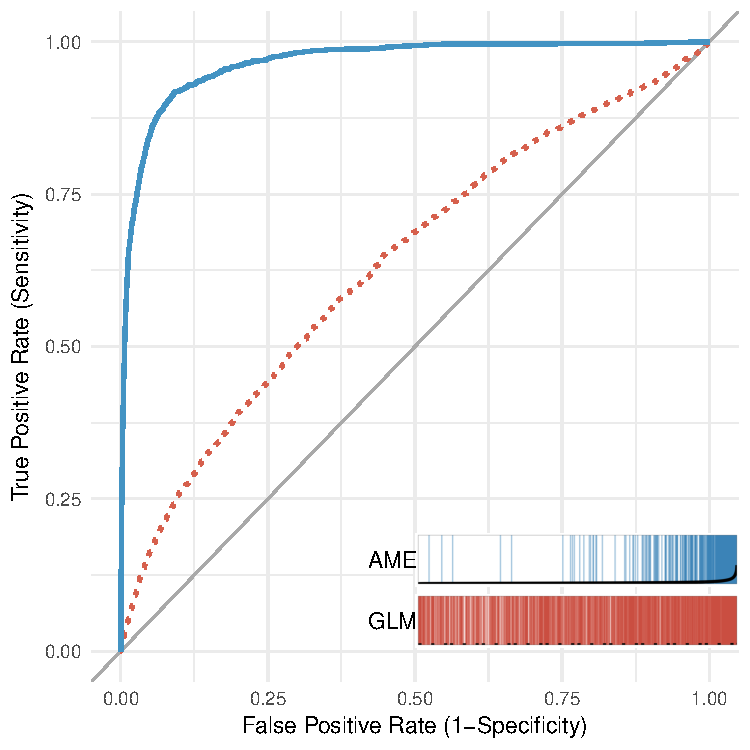
\includegraphics[width=.45\textwidth]{weeks_roc_outSample.pdf}}
	\subfigure[Precision and Recall]{\label{fig:reitpr}\includegraphics[width=.45\textwidth]{weeks_pr_outSample.pdf}}
	\caption{Assessments of out-of-sample predictive performance for Weeks (2012) using ROC curves and PR curves}
\end{figure}
\FloatBarrier

\subsection{Replication of Gibler (2017)}


The replications we have undertaken are all from articles over the past fifteen years.  A more recent example is \citet{gibler:2017} which examines the onset of militarized disputes using capabilities, joint democracy, alliances, and power parity in a undirected dyadic study using logistic regression and dyad clustered standard errors.   In addition to this, Gibler shows that the long-standing relationship between the relative parity of capabilities and initiation of international conflict is almost completely mediated by the initial conditions for the members of the dyad when they joined the international system as sovereign members. This finding calls into question many IR theories about the role of balance in terms of generating international conflict \citep{organski:1958}.


Insert coefplot here, without splines...\label{fig:giberrepl}
%
%\begin{table}
%\begin{center}
%\caption{Comparison of Gibler (2017) Model 6 results with AME results. This was run over a chain of $10,000 \text{BAZILLION}$ iterations.  \label{tab:gibme}}
%\begin{tabular}{lrr} \toprule
%& \multicolumn{2}{c}{$\hat{\beta}$ Estimates}\\ \cmidrule{2-3}
%Variable & \texttt{logit} & \texttt{amen} \\ \midrule
%Allied & 0.142&  0.023 \\
%Joint Democracy &\bf -0.507&  0.045 \\
%Peace Years \bf &-0.260& \bf -0.060 \\
%Spline 1 &\bf -0.001& \bf 0.00 \\
%Spline 2&\bf -0.000& \bf 0.00\\
%Spline 3 &-0.000& \bf 0.00\\ 
%Contiguity &\bf 2.412& \bf 0.640 \\
%Parity &0.075&  -0.013 \\
%Parity at entry year&\bf 0.868&  0.002 \\ 
%Rivalry &\bf 2.031&\bf 0.721\\ 
%Constant &\bf -5.526 & \bf  -2.581\\ \bottomrule
%\end{tabular}\\
%\end{center}
%{\bf Note}: {\bf Bold} indicates conventional statistical significance at $p < 0.05$ or less in Gibler (2017). For comparative purposes, only, we have employed the same criterion to the results from the \texttt{amen} estimation. NEED TO BE FIXED if staying.
%\end{table}

We re-estimated model 6 from Table 6 (2017, 34). The results are presented in Figure~\ref{fig:giberrepl} in order to facilitate explicit comparison.
The results obtained with \texttt{amen} stand in stark contrast to those found with a logistic regression (with dyad clustered, robust standard errors).  Most importantly, the primary variable from the Gibler study, parity of the members of a dyad at the year in which they entered the international system, is shown to be unimportant in the AME results.  Not only is the value of this parameter small, but it has a very large relative standard error -- over a magnitude larger than the parameter itself ($z= 0.038$). In addition, the variable indicating whether both members of the dyad were coded as democracies (joint democracy) follows the same pattern: important and strong in the logistic results, but this disappears once interdependencies are modeled.  As might be expected, the strong geographic clustering in the original study is about one-quarter as strong in the AME estimations. Similarly, rivalry coefficients are about one-third the size in the AME formulation, but a great deal more precisely measured ($z=18.116$). 

We utilized the original and the AME results from Gibler's model 6 in Table 6 to calculate the expected values for one scenario. We focused on the variables measuring rivalry.  We used mean or modal values for all independent variables, except we changed the rivalry variable to indicate that there was a rivalry when the actual data suggest there is none.  The expected values of this scenario are essentially a first difference plot comparing results with the model when estimated in two different ways: Gibler's GLM estimation and our AME approach.  As this Figure~\ref{fig:gibmargeff} illustrates, the AME results differ from the GLM in two distinct ways. First, the expected value of the dependent variable -- the probability of the onset of a militarized interstate dispute, is considerably higher when taking interdependencies into account with the AME model.  These are rare events, so the probabilities are low, but the difference is a factor of $3x$. Thus, you get quite substantially different expected values from these two models.  Second, the GLM model has a standard errors which underestimate the true variability, in part because some of them are assumed to be zero.  This shows up in the narrow density of predicted outcomes for the GLM model, compared to the density seen with the AME. The latter reflects a wider range of potential outcomes, reflecting the incorporation of uncertainty in the AME model.

\begin{figure}
	\caption{THIS NEEDS TO BE FIXED.  \label{fig:gibmargeff}}
	\includegraphics[width=\textwidth]{gibler_margeff.pdf}
 	\label{fig:gibmargeff}
 \end{figure}

Beyond more informative fixed-effects coefficients, the AME approach also provides information about the interdependencies that were modeled. The assumption of independence among the dyadic data in this study can be strongly rejected. Perhaps most importantly, the main substantive conclusions of the 2017 Gibler study do not seem warranted from the perspective of the results obtained with the \texttt{amen} estimation that explicitly models \first- \second-, and \third-order interdependencies. Not only do the estimated coefficients tell a different story, but the assumptions under which the original results would hold are shown to be violated by the data.

\subsection{Lessons Learned from Re-estimating Five Prominent Studies}

First and foremost, many  findings which emerge from models that do not take interdependencies into account lose their statistical significance when network effects are estimated via AME. This should not be news -- since the finding has long been in the theoretical literature, but given the state of current literature in international relations is still pertinent.  Not only
are coefficients biased in the OLS and logit approaches to the analysis of dyadic data, but they are often imprecisely measured, with inflated standard errors.  This means that significant testing (for better or worse) is compromised when network effects are ignored.

Second, even when the results from the AME estimation conform with those found in an OLS or logistic regression, new insights
emerge from the additional information derived. In particular, there is actual information about the dependencies so that clusters can be identified, and the extent of reciprocity at the dyad level, as well as among senders and receivers.  This kind of information
is absent in standard approaches and add to our ability to explain specific as well as general results.

Third, it is evident that the actual results -- not the estimated coefficents and their covariances -- which are generated by the models differ greatly in expectations.  This implies that policy experimentations with the models, as well as scenario-based simulations and forecasting of GLM models are likely to often give misleading results compared to the AME approach.

Fourth, it is clear that the AME approach dominates the OLS and Logit-based approaches in terms of performance. Not only it is better at correctly identifying cases in which the dependent variable takes a value of $0$ (via the ROC curves and associated statistics), but it also dominates at correctly identifying occurrences of the dependent variable in the data (seen via the PR curves and associated statistics).  In the case of studies
with continuous dependent variables, the AME approach has average error statistics that are about one-half that found in the OLS model. It is rare for studies in this area to provide performance statistics, but at the same time that at least one of the studies is unable to identify a single case in spite of having almost a million observations.

Fifth, it is useful to suggest that a lot of what is \textit{known} about international relations based on studies of dyadic data should be taken with a grain of salt, and awaits a reassessment using methods that do not rely on an assumption that all the dyads are independent and identically distributed.



\section{\textbf{Conclusion}}

International relations is generally about the interactions and dependencies among a set of countries or other important actors such as international governmental organizations (IGOs). This is particularly true of scholarship in the tradition of the Correlates of War Project, but it is by no means limited to it.\footnote{See \cite{singer:1972} for an early description of the project and also see the project's Web site for an history and more recent efforts \url{http://www.correlatesofwar.org/}.} Many scholars have debated the use and abuse of dyadic data.\footnote{One recent on-line symposium can be found at \url{http://bit.ly/2wB2hab}.} It is clear from a survey of the literature and from work in this area published as recently as 2017 that many find dyadic data to be an important touchstone in the study of international relations \citep{erikson:pinto:2014,aronow:etal:2015}.

At the same time, we know that research designs focusing on the statistical analysis of dyadic data quickly go astray if the dyadic data are assumed to be iid.  Virtually all of the standard statistical models---ordinary least squares and logistic regressions, to name a few---fail if the data are not conditionally independent. This fact has been accepted when it comes to temporal dependencies, but adoption of methods to account for network dependencies have seen less progress. By definition dyadic data are not iid and thus the standard approaches can not be used cavalierly to analyze these data.  \citet{signorino:1999} showed why this is true of models of strategic interaction, but it is more broadly true of models that employ dyadic data.  We show that the AME framework can be employed to account for the statistical issues that arise when studying dyadic data.

To explore this approach in the context of international relations we have presented two broad analyses. The first is a simulation where the characteristics of the network are known. This shows that when there are unobserved dependencies, the AME approach is less biased in terms of parameter estimation compared to the standard approach employed in international relations to study dyadic data (i.e., GLM models). The second analysis is a replication of recent studies that have been published recently using a broad range of dyadic data to draw inferences about international relations.  These studies have been replicated with the original research designs, each of which used a statistical method that assumes the dyadic data are all independent from one another.  We then re-analyzed each study using the AME model.  In every case, we found that the AME approach provided a) increased precision of estimation, b) better out-of-sample fit, and c) evidence of 1st-, 2nd-, and 3rd-order dependencies that were overlooked in the original studies.\footnote{The Appendix contains performance data on all of these replications, as well as sample code illustrating how to undertake AME analysis using \texttt{amen}.} In several cases, the new approach overturns the basic findings of the original research.

It is no longer necessary to assume that the interesting, innate interdependencies in relational data about international relations can be ignored. Nor do they have to be approximated with \textit{ad hoc}, incomplete solutions that purport to control for dependencies (such as modifying the post-estimation standard errors of the estimated coefficients \citep{king:roberts:2014}). Instead, the interdependencies may be addressed directly with additive and multiplicative effects in the context of a generalized linear model that provides more reliable inferences, better out-of-sample predictive performance, and new substantive insights. 
\appendix
\clearpage

\renewcommand{\thefigure}{A\arabic{figure}}
\setcounter{figure}{0}
\renewcommand{\thetable}{A.\arabic{table}}
\setcounter{table}{0}
\renewcommand{\thesection}{A.\arabic{section}}
\setcounter{section}{0}

\section*{\textbf{Appendix}}

% \subsection*{}

% \subsection*{Additive and Multiplicative Effects Gibbs Sampler}

% To estimate, the effects of our exogenous variables and latent attributes we utilize a Bayesian probit model in which we sample from the posterior distribution of the full conditionals until convergence. Specifically, given observed data $\textbf{Y}$ and $\textbf{X}$ -- where $\textbf{X}$ is a design array that includes our sender, receiver, and dyadic covariates -- we estimate our network of binary ties using a probit framework where: $y_{ij} = 1(\theta_{ij}>0)$ and $\theta_{ij} = \bm\beta^{\top}\mathbf{X}_{ij} + a_{i} + b_{j} + \textbf{u}_{i}^{\top} \textbf{D} \textbf{v}_{j} + \epsilon_{ij}$. 

% \begin{itemize}
%  \item Given initial values of $\{\bm\beta, \textbf{a}, \textbf{b}, \textbf{U}, \textbf{V}, \Sigma_{ab}, \rho, \text{ and } \sigma_{\epsilon}^{2}\}$, the algorithm proceeds as follows:
%  \begin{itemize}
%  	\item sample $\bm\theta \; | \;  \bm\beta, \textbf{X}, \bm\theta, \textbf{a}, \textbf{b}, \textbf{U}, \textbf{V}, \Sigma_{ab}, \rho, \text{ and } \sigma_{\epsilon}^{2}$ (Normal)
%  	\item sample $\bm\beta \; | \;  \textbf{X}, \bm\theta, \textbf{a}, \textbf{b}, \textbf{U}, \textbf{V}, \Sigma_{ab}, \rho, \text{ and } \sigma_{\epsilon}^{2}$ (Normal)
%  	\item sample $\textbf{a}, \textbf{b} \; | \; \bm\beta, \textbf{X}, \bm\theta, \textbf{U}, \textbf{V}, \Sigma_{ab}, \rho, \text{ and } \sigma_{\epsilon}^{2}$ (Normal)
% 	\item sample $\Sigma_{ab} \; | \; \bm\beta, \textbf{X}, \bm\theta, \textbf{a}, \textbf{b}, \textbf{U}, \textbf{V}, \rho, \text{ and } \sigma_{\epsilon}^{2}$ (Inverse-Wishart)
%  	\item update $\rho$ using a Metropolis-Hastings step with proposal $p^{*} | p  \sim$ truncated normal$_{[-1,1]}(\rho, \sigma_{\epsilon}^{2})$
%  	\item sample $\sigma_{\epsilon}^{2} \; | \; \bm\beta, \textbf{X}, \bm\theta, \textbf{a}, \textbf{b}, \textbf{U}, \textbf{V}, \Sigma_{ab}, \text{ and } \rho$ (Inverse-Gamma)
%  	\item For each $k \in K$:
%  	\begin{itemize}
%  		\item Sample $\textbf{U}_{[,k]} \; | \; \bm\beta, \textbf{X}, \bm\theta, \textbf{a}, \textbf{b}, \textbf{U}_{[,-k]}, \textbf{V}, \Sigma_{ab}, \rho, \text{ and } \sigma_{\epsilon}^{2}$ (Normal)
%  		\item Sample $\textbf{V}_{[,k]} \; | \; \bm\beta, \textbf{X}, \bm\theta, \textbf{a}, \textbf{b}, \textbf{U}, \textbf{V}_{[,-k]}, \Sigma_{ab}, \rho, \text{ and } \sigma_{\epsilon}^{2}$ (Normal)
%  		\item Sample $\textbf{D}_{[k,k]}  \; | \; \bm\beta, \textbf{X}, \bm\theta, \textbf{a}, \textbf{b}, \textbf{U}, \textbf{V}, \Sigma_{ab}, \rho, \text{ and } \sigma_{\epsilon}^{2}$ (Normal)\footnote{Subsequent to estimation, \textbf{D} matrix is absorbed into the calculation for $\textbf{V}$ as we iterate through $K$. }
%  	\end{itemize}
%  \end{itemize}
% \end{itemize}


\newpage
% Bib stuff
\clearpage

%\bibliography{/Users/maxgallop/documents/whistle/master}
\bibliography{/Users/s7m/whistle/master}
% \bibliography{/Users/mdw/Git/whistle/master}
% \bibliography{/Users/cassydorff/ProjectsGit/master}
% \bibliographystyle{authordate1}
\bibliographystyle{sm}
% \clearpage
% \section*{All About Us}

\end{document}
